\documentclass{article}

\usepackage{tikz}
\usetikzlibrary{automata}

\begin{document}

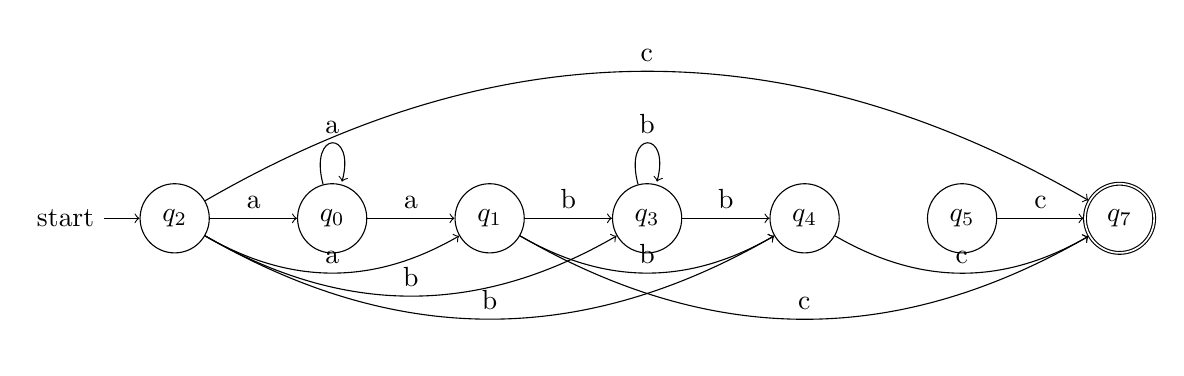
\begin{tikzpicture}[->, auto, node distance = 2cm]
\node[initial,state] (q2) {$q_{2}$};
\node[state] (q0) [right of=q2] {$q_{0}$};
\node[state] (q1) [right of=q0] {$q_{1}$};
\node[state] (q3) [right of=q1] {$q_{3}$};
\node[state] (q4) [right of=q3] {$q_{4}$};
\node[state] (q5) [right of=q4] {$q_{5}$};
\node[state,accepting] (q7) [right of=q5] {$q_{7}$};

\path (q0) edge node {a} (q1);
\path (q0) edge [loop above] node {a} (q0);
\path (q2) edge [bend right] node {a} (q1);
\path (q2) edge node {a} (q0);
\path (q2) edge [bend right] node {b} (q4);
\path (q2) edge [bend right] node {b} (q3);
\path (q2) edge [bend left] node {c} (q7);
\path (q1) edge [bend right] node {b} (q4);
\path (q1) edge node {b} (q3);
\path (q1) edge [bend right] node {c} (q7);
\path (q3) edge node {b} (q4);
\path (q3) edge [loop above] node {b} (q3);
\path (q4) edge [bend right] node {c} (q7);
\path (q5) edge node {c} (q7);
\end{tikzpicture}

\end{document}